\section{Planning and Paperwork}

The \pbproleref{role:race_org_team} should prepare a few potential routes for each event,
typically using software like Trailforks or MapMyRide as shown in \reffig{road_pbp_trailforks}.

\begin{figure}[h]
  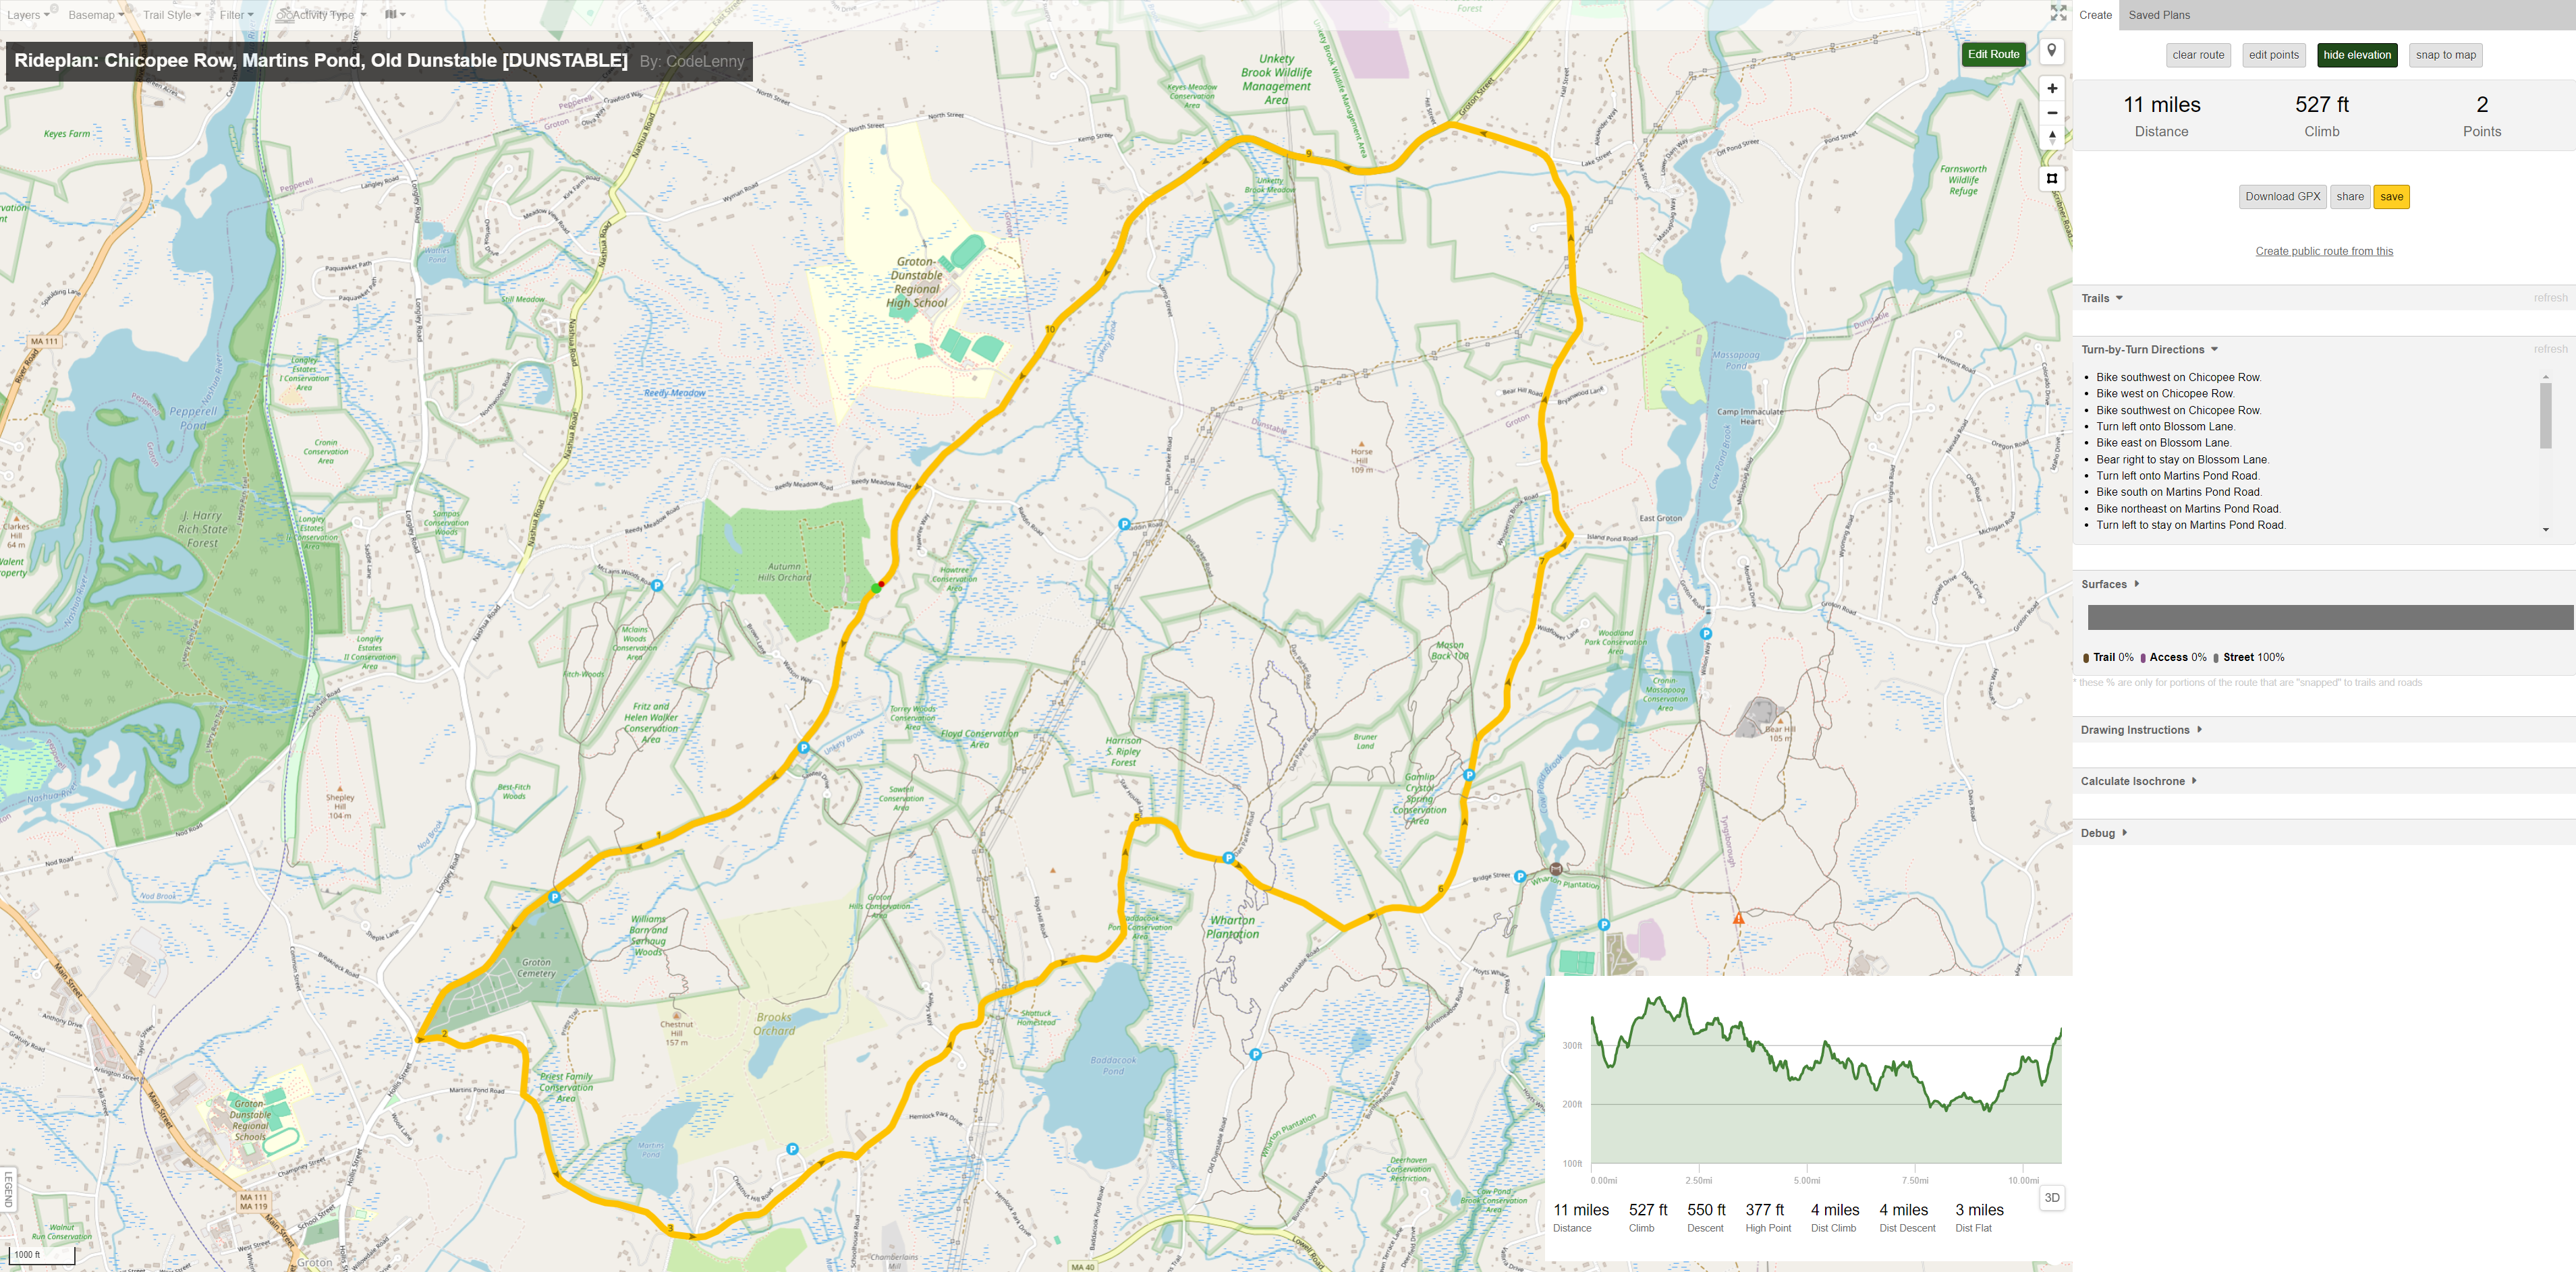
\includegraphics[width=1\textwidth]{2024_groton_trailforks.png}
  \caption[Road race course map in Trailforks]{
    A potential road race course in Groton, MA
    prepared via Trailforks for the 2024 Road Season.\\
    Credit: Flyyn Leonard}
  \labfig{road_pbp_trailforks}
\end{figure}

The \pbproleref{role:lead_org} should contact the local town or city
to determine what permits may be required, and make an initial contact to the police department,
as the police are typically a critical component to planning and running the race.

Once the race has passed the initial hurdle of getting a route and hasn't been shot down by the local government,
the \pbproleref{role:race_org_team} should evaluate local services and get quotes for:

\begin{itemize}
  \item Medical coverage, often by the local fire department or contracted private ambulance service
  \item Barriers and other course supplies - these may be supplied by the local police or highway department, or rented from private companies
\end{itemize}

The \pbproleref{role:eccc_coordination_team} is available to help and advise the organizing team throughout this entire process,
and can often provide suggestions of who to contact, and have a list of departments and private companies that have been used in the past.

\subsection{Budget}

Using all of the information gathered in the initial planning phase, the \pbproleref{role:race_org_team} should start drafting a race budget
to ensure the race will be financially viable.

A sample budget is included in \nrefch{event_budget}, and teams can contact the \pbproleref{role:eccc_coordination_team}
for a digital copy of the ECCC race budget template.
Using the official ECCC budget format is preferred, allowing ECCC staff to easily compile and compare budgets across weekends and years.

Teams should contact the \pbproleref{role:eccc_coordination_team} to discuss what registration fees should be for the entire season -
the ECCC tries to keep registration fees consistent across all races of the season, which makes it easy for teams to register.

\subsection{Flyer Design}

Once the race is deemed viable, the \pbproleref{role:race_org_team} should prepare a flyer, working with the \pbproleref{role:eccc_coordination_team}
to ensure the flyer meets the standard format dictated by the USA Cycling permitting process as well as the ECCC standards.

The race flyer is critical to obtaining a USA Cycling event permit.

\subsection[USA Cycling Permitting]{Obtaining a USA Cycling Permit}

Working with the \pbproleref{role:eccc_coordination_team}, the \pbproleref{role:lead_org} should submit a USA Cycling event permit application.

Once approved, this will provide Certificates of Insurance (COI) % TODO: add to glossary
typically required by the local government,
and should automatically start the process of getting USA Cycling Officials to work the event.
